\begin{mdframed}[style=warning]
	\begin{ejercicio}
		Una partícula de masa $m$, cuya velocidad inicial es $v_o$ sujeta a una fuerza $F(t)$ como se ve en la figura \ref{ej1}. \textbf{(a)} Realize un bosquejo del comportamiento esperado de $v(t)$ y $x(t)$. \textbf{(b)} Cree una función simple (utilizando la gráfica) y encuentre $v(t)$ y $x(t)$.
		\begin{figure}[H]
			\centering
			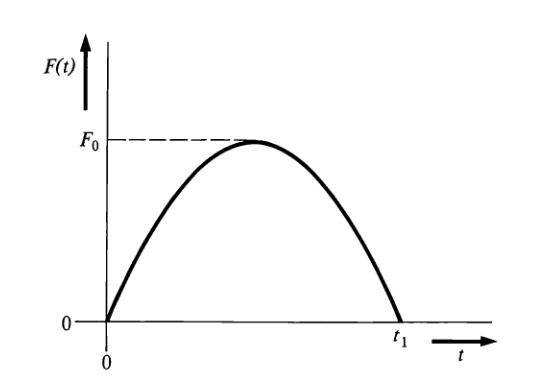
\includegraphics[scale=0.3]{img/ej1.png}
			\caption{Problema 1}
			\label{ej1}
		\end{figure}
	\end{ejercicio}
\end{mdframed}



\begin{mdframed}[style=warning]
	\begin{ejercicio}
		Una partícula se mueve en un medio bajo la influencia de una fuerza de retardo igual a $mk(v^3 + a^2 v)$, donde $k$ y $a$ son constantes. Muestre que para cualquier valor inicial la velocidad de la partícula nunca se moverá a una distancia mayor a $\flatfrac{\pi}{2ka}$ y que la partícula llega al reposo sólo cuando $t\to \infty$.
	\end{ejercicio}
\end{mdframed}

\begin{mdframed}[style=warning]
	\begin{ejercicio}
		La expresión de Prandtl para la resistencia del aire es:
			$$ W = \frac{1}{2} c_W \rho A v^2 $$
		donde $c_W$ es una constante de arrastre adimensional, $\rho$ es la resistencia del aire, $v$ es la velocidad y $A$ es la sección transversal del objeto medida perpendicularmente a la velocidad.
		
		Un jugador de softball batea una pelota a $0.7m$ del suelo. La pelota inicia su trayectoria con ángulo de $35^o$ y viaja hacia una barda de $2m$ de alto que se encuentra a $60m$ de donde se encuentra el jugador. El coeficiente de arrastre del aire es $c_W = 0.5$, el radio de la pelota $r = 5cm$ y la masa de $200g$. Considerando que la resistencia del aire es proporcional al cuadrado de la velocidad de la pelota,
		\begin{enumerate}[a)]
			\item Encuentre la velocidad inicial que la pelota necesita para salvar la barda. Considere que la densidad del aire es de $1.3 kg/m^3$. Realice una gráfica $x-y$ comparando la trayectoria considerando resistencia del aire y también la trayectoria sin considerarla.
			\item Considerando la velocidad inicial calculada en el inciso anterior, calcule el ángulo de elevación que se debiera imprimir a la pelota para que la altura por encima de la barda sea máxima. ¿Cuál es el valor de esa altura?
		\end{enumerate}
	\end{ejercicio}
\end{mdframed}